\documentclass{acmart}
\usepackage[english]{babel}
\usepackage{hhline}
\usepackage{multirow}
\usepackage{graphicx}
\graphicspath{ {./images/} }
\usepackage{caption}
\usepackage{sidecap}
\usepackage{titlesec}
\usepackage{hyperref}



\begin{document}
\begin{titlepage}
    \title{Query Image Modification}
    \author{Astafev, Dmitriev}
    

    \maketitle
\end{titlepage}

\tableofcontents
\newpage
\section{Query Image Modification}
\subsection{Query Image Modification}
As mentioned earlier, a user may select one or more segments of interest by clicking on them. We handle these two cases separately since Boolean AND/OR alone is not sufficient to describe multiple segments. Often, there is a semantic relationship between the segments of interest since the segmentation algorithm generally does not segment semantic objects in an image as a single segment. A user may, thus, select multiple segments to capture her notion of the query object. For example, a color-based segmentation will segment a multi-color national flag into multiple segments, and thereby destroying the object semantics. We next describe the heuristics used to generate the modified images for both single and multiple segment cases and discuss how the user perception is learnt from the user’s response on these modified images. (Figure \ref{fig:1}.)
\begin{enumerate}
    \item  	Multiple Segment Modification 
    \item   The purpose behind multiple-segment modification is to estimate the relative importance of the spatial relationships, and query expansion, if needed. This helps in determining what best describes the user perception in a multiple segment-query. Independent modifications of features of each segment generate a large number of modified images. The user will not have the patience for providing feedback on these modified images. Such mindless modifications will even confuse the user leading to incoherent feedback on his part. Additionally, many of the modified images will not even help in estimating the retrieval parameters. So we utilize the concept of a semantic object for pruning the set of modifications. Frequently, when the user selects multiple segments of interest, these form a semantic object, where different segments satisfy some spatial constraints. A semantic object represents a group of segments whose relative shape, size and spatial organization as a whole defines the user's notion of query object. For example, when a user selects the multiple segments of a multi-color flag, generating independent modifications for these segments is not at all efficient for learning the retrieval parameters.(Form \ref{form})
    \item Manipulation of Segment Contiguit
    \item Let M be the number of selected segments by the user. Define an incidence matrix of size $ M \times M$
    \begin{equation}
        C=[{c_i}_j]+\lim_{n \to -\infty}\left(1+\frac{1}{i}\right)^n\label{form}
    \end{equation}
    \item A scheme for reducing contiguity between M segments Figure \ref{fig:1}. Segments of interest form a triangular shape in the query image. of interest is given below.
    
    \item Identify any noncontiguous segment i by finding. Remove i-th row and column of the incident matrix C. Decrement M.
    
    \item Find maximally contiguous segment (Figure \ref{fig:2}.)
    \begin{center}
    $A = \sum\limits_{i=1}^n(z+v)\dfrac{a^i }{bc^j} + \lim\limits_{n \to -\infty}\left(1+\dfrac{1}{i}\right)^n$
    \end{center} 
    \item If more than one exist, choose the larger. In case of a tie, choose a segment randomly.
    \item Compute the convex hull of the remaining (M-1) segments. Move the maximally contiguous segment outside the convex hull.
    
\begin{center}
        $\sum\limits_{i=0}^n \int\limits_i^j \dfrac{{c_i}_j}{\lim\limits_{n \to 8}n} + \sqcap{_j}i \times j_i
    $
    \end{center} 
    \item Remove the ifrom the matrix C.  Otherwise go to (2).
\end{enumerate}
\begin{figure}
    \begin{center}
    \centering
    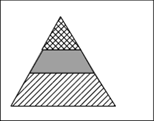
\includegraphics{1.png}
    \caption{Segments of interest form a triangular shape in the query image.}
    \label{fig:1}
    \end{center}
\end{figure}

\begin{figure}
    \begin{center}
    \centering
    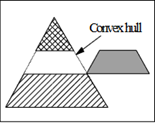
\includegraphics{2.png}
    \caption{Segments of interest form a triangular shape in the query image.}
    \label{fig:2}
    \end{center}
\end{figure}



\subsection*{Steps:}
\begin{itemize}
    \item 	Segments of interest form a triangular shape in the query image. (Table \ref{tbl:1})
    \item 	Selected segments scaled down about their centroids.
    \item 	Segments scaled down about their contact points with the maximally contiguous segment.
\end{itemize}

    \begin{center}
    \begin{tabular}{|c|c|c|c|c|c|c|c|c|}
            
        
        \hline
         
         &\multicolumn{4}{c}{Relevance feedback}& \multicolumn{3}{c}{Intra-query } &\\
         \hline
       Interation & 0 &1 &3 &6 &0 &1 &2 &3 \\
       \hline
       N &13 &18 &20 &23 &19 &22 &22 &23 \\
       \hline
    \end{tabular}
    \captionof{table}{Performance comparison of intra-query learning and relevance feedback}
    \label{tbl:1}
    \end{center}

\newpage
\newpage
\addcontentsline{toc}{section}{DISCUSSIONS}
\section*{DISCUSSIONS}

The goal of the CBIR engine is to retrieve other images from the image database, which the user perceives as close to the query image in the high-dimensional space corresponding to the low-level description of the image. Existing relevance feedback approaches have attempted pruning of the high-dimensional space through user feedback on the database retrieval results. Our approach fundamentally differs from these in that it prunes the highdimensional space through user feedback on various query-point modifications in this space, without any database access.

\newpage
\addcontentsline{toc}{section}{REFERENCES}
\section*{REFERENCES}


1	J.R. Bach, C. Fuller, A. Gupta, et al. The Virage image search engine: An open framework for image management. In Proceedings of the SPIE Storage and Retrieval for Image and Video Databases, 2670, San Jose, U.S.A., 1996.
2	C. Carson, S. Belongie, H. Greenspan, et al. Region-based image querying. In Proceedings of the IEEE Workshop on Content-Based Access of Image and Video Libraries, San Juan, Puerto Rico, 1997.
3	D. Comaniciu, and P. Meer. Robust Analysis of feature spaces: Color image segmentation. In Proceedings of the IEEE Conference on Computer Vision and Pattern Recognition, San Juan, Puerto Rico, 1997
4	I.J. Cox, M.L. Miller, T.P. Minka, et al. An optimized interaction strategy for Bayesian relevance feedback. In Proceedings of the IEEE Conference on Computer Vision and Pattern Recognition, Santa Barbara, U.S.A., 1998.
5	M. Flickner, H. Sawhney, W. Niblack, et al. Query by image and video content: The QBIC system. IEEE Computer 28(9):23-32, Sept 1995.




\end{document}
